\documentclass [15pt,a4paper,twoside]{article}
\usepackage[english,shorthands=off]{babel}        % shorhands=off is required for babel french in combination with tikz karnaugh....
\usepackage[utf8x]{inputenc}
\usepackage[T1]{fontenc}
\usepackage{amsmath}
\usepackage{geometry}
\geometry{verbose,a4paper, tmargin=3.5cm,bmargin=3.5cm,lmargin=2.5cm,rmargin=2.5cm,headsep=1cm,footskip=1.5cm}
\usepackage{fancyhdr}
\usepackage{colortbl}
\usepackage[dvipsnames]{xcolor}
\usepackage{tikz -timing}
\usepackage{tikz}
\usetikzlibrary{karnaugh}
\pagestyle{fancy}

\definecolor{LogisimKMapColor0}{RGB}{128,0,0}
\definecolor{LogisimKMapColor1}{RGB}{230,25,75}
\definecolor{LogisimKMapColor2}{RGB}{250,190,190}
\definecolor{LogisimKMapColor3}{RGB}{170,110,40}
\definecolor{LogisimKMapColor4}{RGB}{245,130,48}
\definecolor{LogisimKMapColor5}{RGB}{255,215,180}
\definecolor{LogisimKMapColor6}{RGB}{128,128,0}
\definecolor{LogisimKMapColor7}{RGB}{255,255,25}
\definecolor{LogisimKMapColor8}{RGB}{210,245,60}
\definecolor{LogisimKMapColor9}{RGB}{0,0,128}
\definecolor{LogisimKMapColor10}{RGB}{145,30,180}
\definecolor{LogisimKMapColor11}{RGB}{60,180,175}
\definecolor{LogisimKMapColor12}{RGB}{0,130,203}
\definecolor{LogisimKMapColor13}{RGB}{230,190,255}
\definecolor{LogisimKMapColor14}{RGB}{170,255,195}
\definecolor{LogisimKMapColor15}{RGB}{240,50,230}

\fancyhead{}
\fancyhead[C] {Logisim-evolution generated document on Fri Jul 23 12:11:45 CLT 2021}
\fancyfoot[C] {\thepage}
\renewcommand{\headrulewidth}{0.4pt}
\renewcommand{\footrulewidth}{0.4pt}

\makeatother

\begin{document}
\section{Introduction}
This document was generated by logisim-evolution. Any part of the TeX sources can be used in your own documents without any problems. In case you want to use all/parts of this generated TeX-sources please (1) do not forget to include the required packages, and (2) include a remark that this source was generated by logisim-evolution.
%===============================================================================
\section{Truth table}
The table may be way to big to be displayed on the page. At generation time no calculation was done on the size of the table with respect to the width/height of the page.
%-------------------------------------------------------------------------------
\subsection{Compacted truth table}
\begin{center}
\begin{tabular}{cc|c}
$A$&$B$&$Y$\\
\hline
$0$&$0$&$0$\\
$0$&$1$&$1$\\
$1$&$0$&$1$\\
$1$&$1$&$0$\\

\end{tabular}
\end{center}
%-------------------------------------------------------------------------------
\subsection{Complete truth table}
\begin{center}
\begin{tabular}{cc|c}
$A$&$B$&$Y$\\
\hline
$0$&$0$&$0$\\
$0$&$1$&$1$\\
$1$&$0$&$1$\\
$1$&$1$&$0$\\

\end{tabular}
\end{center}
%===============================================================================
\section{Karnaugh diagrams}
This section shows various versions of the Karnaugh diagrams of the given functions.
%-------------------------------------------------------------------------------
\subsection{Empty Karnaugh diagrams}
\begin{center}
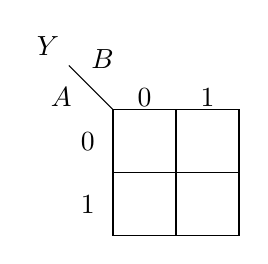
\begin{tikzpicture}[karnaugh,disable bars,x=1\kmunitlength,y=1\kmunitlength,kmbar left sep=1\kmunitlength,grp/.style n args={4}{#1,fill=#1!30,minimum width= #2\kmunitlength,minimum height=#3\kmunitlength,rounded corners=0.2\kmunitlength,fill opacity=0.6,rectangle,draw}]
\karnaughmap{2}{$Y$}{{$A$}{$B$}}{}{
\draw[kmbox] (-0.5,2.5)
   node[below left]{$A$}
   node[above right]{$B$} +(-0.2,0.2)
   node[above left]{$Y$};\draw (0,2) -- (-0.7,2.7);
\foreach \x/\1 in %
{0/0,1/1} {
   \node at (\x+0.5,2.2) {\1};
}
\foreach \y/\1 in %
{0/0,1/1} {
   \node at (-0.4,-0.5-\y+2) {\1};
}
}
\end{tikzpicture}
\end{center}
%-------------------------------------------------------------------------------
\subsection{Filled in Karnaugh diagrams}
\begin{center}
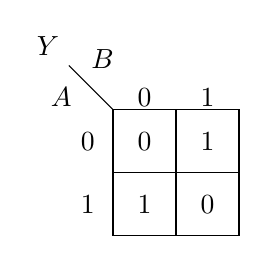
\begin{tikzpicture}[karnaugh,disable bars,x=1\kmunitlength,y=1\kmunitlength,kmbar left sep=1\kmunitlength,grp/.style n args={4}{#1,fill=#1!30,minimum width= #2\kmunitlength,minimum height=#3\kmunitlength,rounded corners=0.2\kmunitlength,fill opacity=0.6,rectangle,draw}]
\karnaughmap{2}{$Y$}{{$A$}{$B$}}
{0110}{
\draw[kmbox] (-0.5,2.5)
   node[below left]{$A$}
   node[above right]{$B$} +(-0.2,0.2)
   node[above left]{$Y$};\draw (0,2) -- (-0.7,2.7);
\foreach \x/\1 in %
{0/0,1/1} {
   \node at (\x+0.5,2.2) {\1};
}
\foreach \y/\1 in %
{0/0,1/1} {
   \node at (-0.4,-0.5-\y+2) {\1};
}
}
\end{tikzpicture}
\end{center}
%-------------------------------------------------------------------------------
\subsection{Filled in Karnaugh diagrams with covers}
\begin{center}
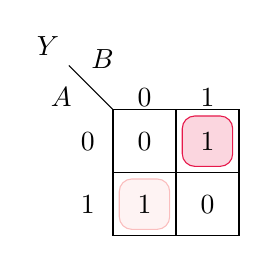
\begin{tikzpicture}[karnaugh,disable bars,x=1\kmunitlength,y=1\kmunitlength,kmbar left sep=1\kmunitlength,grp/.style n args={4}{#1,fill=#1!30,minimum width= #2\kmunitlength,minimum height=#3\kmunitlength,rounded corners=0.2\kmunitlength,fill opacity=0.6,rectangle,draw}]
\karnaughmap{2}{$Y$}{{$A$}{$B$}}
{0110}{
\draw[kmbox] (-0.5,2.5)
   node[below left]{$A$}
   node[above right]{$B$} +(-0.2,0.2)
   node[above left]{$Y$};\draw (0,2) -- (-0.7,2.7);
\foreach \x/\1 in %
{0/0,1/1} {
   \node at (\x+0.5,2.2) {\1};
}
\foreach \y/\1 in %
{0/0,1/1} {
   \node at (-0.4,-0.5-\y+2) {\1};
}
   \node[grp={LogisimKMapColor1}{0.8}{0.8}](n0) at(1.5,1.5) {};
   \node[grp={LogisimKMapColor2}{0.8}{0.8}](n1) at(0.5,0.5) {};
}
\end{tikzpicture}
\end{center}
%===============================================================================
\section{Minimal expressions}
$Y =  \overline{A}  \cdot B+A \cdot  \overline{B} $~\\
\end{document}
